\whiteBGstarBegin
\setcounter{section}{0}
\section{Trắc nghiệm}
\begin{enumerate}[label=\bfseries Câu \arabic*:]
	
	
	\item \mkstar{1}
	
	\cauhoi
	{Việc ghép nối tiếp các nguồn điện thì sẽ tạo thành một bộ nguồn mới có
		\begin{mcq}
			\item suất điện động lớn hơn các nguồn có sẵn.
			\item suất điện động nhỏ hơn các nguồn có sẵn.
			\item điện trở trong nhỏ hơn các nguồn có sẵn.
			\item điện trở trong bằng điện trở ngoài.
		\end{mcq}
		
	}
	\loigiai
	{	\textbf{Đáp án: A.}
		
		Việc ghép nối tiếp các nguồn điện thì sẽ tạo thành một bộ nguồn mới có suất điện động lớn hơn các nguồn có sẵn.
		$$\calE = \calE_1 + \calE_2 + \ldots + \calE_n.$$
	}
	\item \mkstar{1}
	
	\cauhoi
	{Việc ghép song song các nguồn điện giống nhau thì sẽ tạo thành một bộ nguồn mới có
		\begin{mcq}
		\item suất điện động lớn hơn các nguồn có sẵn.
		\item suất điện động nhỏ hơn các nguồn có sẵn.
		\item điện trở trong nhỏ hơn các nguồn có sẵn.
		\item điện trở trong bằng điện trở ngoài.
		\end{mcq}
		
	}
	\loigiai
	{	\textbf{Đáp án: C.}
		
		Việc ghép song song các nguồn điện giống nhau thì sẽ tạo thành một bộ nguồn mới có điện trở trong nhỏ hơn các nguồn có sẵn.
		$$r=\dfrac{r_1 r_2 \ldots r_n}{r_1 + r_2 + \ldots + r_n} = \dfrac{r^n}{nr}.$$
	}
	\item \mkstar{2}
	
	\cauhoi
	{Ghép nối tiếp 3 pin giống nhau, mỗi pin có suất điện động 2 V và điện trở trong $\SI{1}{\Omega}$. Suất điện động và điện trở trong của bộ pin là
		\begin{mcq}(2)
			\item $\calE = \SI{6}{V}$ và $r=\SI{3}{\Omega}$.
			\item $\calE = \SI{9}{V}$ và $r=\xsi{1/3}{\Omega}$.
			\item $\calE = \SI{3}{V}$ và $r=\SI{3}{\Omega}$.
			\item $\calE = \SI{3}{V}$ và $r=\xsi{1/3}{\Omega}$.
		\end{mcq}
		
	}
	\loigiai
	{	\textbf{Đáp án: A.}
		
		Khi ghép nối tiếp bộ nguồn thì:
		
		Suất điện động của bộ nguồn:
		$$\calE_\text b= n \calE = \SI{6}{V}.$$
		
		Điện trở trong của bộ nguồn:
		$$r_\text b = nr = \SI{3}{\Omega}.$$
	}
	\item \mkstar{2}
	
	\cauhoi
	{Một mạch điện kín gồm hai nguồn điện $\calE_1$, $r_1$ và $\calE_2$, $r_2$ mắc nối tiếp nhau. Mạch ngoài chỉ có điện trở $R$. Biểu thức cường độ dòng điện trong mạch ngoài là
		\begin{mcq}(2)
			\item $I=\dfrac{\calE_1 - \calE_2}{R+r_1+r_2}$.
			\item $I=\dfrac{\calE_1 - \calE_2}{R+r_1-r_2}$.
			\item $I=\dfrac{\calE_1 + \calE_2}{R+r_1-r_2}$.
			\item $I=\dfrac{\calE_1 + \calE_2}{R+r_1+r_2}$.
		\end{mcq}
		
	}
	\loigiai
	{	\textbf{Đáp án: D.}
		
		Một mạch điện kín gồm hai nguồn điện $\calE_1$, $r_1$ và $\calE_2$, $r_2$ mắc nối tiếp nhau. Biểu thức cường độ dòng điện trong mạch:
		$$I=\dfrac{\calE_1 + \calE_2}{R + r_1 + r_2}.$$
	}
	\item \mkstar{2}
	
	\cauhoi
	{Một mạch điện kín gồm hai nguồn điện $\calE$, $r_1$ và $\calE$, $r_2$ mắc song song với nhau. Mạch ngoài chỉ có điện trở $R$. Biểu thức cường độ dòng điện trong mạch là
		\begin{mcq}(2)
			\item $I=\dfrac{2\calE}{R+r_1+r_2}$.
			\item $I=\dfrac{\calE}{R+\dfrac{r_1 r_2}{r_1 + r_2}}$.
			\item $I=\dfrac{2\calE}{R+\dfrac{r_1 r_2}{r_1 + r_2}}$.
			\item $I=\dfrac{\calE}{R+\dfrac{r_1+r_2}{r_1 r_2}}$.
		\end{mcq}
		
	}
	\loigiai
	{	\textbf{Đáp án: B.}
		
		Một mạch điện kín gồm hai nguồn điện $\calE$, $r_1$ và $\calE$, $r_2$ mắc song song với nhau, mạch ngoài chỉ có điện trở $R$. Biểu thức cường độ dòng điện trong mạch là
		$$I=\dfrac{\calE}{R + \dfrac{r_1 r_2}{r_1 + r_2}}.$$
	}
	\item \mkstar{2}
	
	\cauhoi
	{Một bộ nguồn gồm hai nguồn điện mắc nối tiếp. Hai nguồn có suất điện động lần lượt là 5 V và 7 V. Suất điện động của bộ nguồn là
		\begin{mcq}(4)
			\item 6 V.
			\item 2 V.
			\item 12 V.
			\item 7 V.
		\end{mcq}
		
	}
	\loigiai
	{	\textbf{Đáp án: C.}
		
		Suất điện động của bộ nguồn mắc nối tiếp:
		$$\calE = \calE_1 + \calE_2 = \SI{12}{V}.$$
	}
	\item \mkstar{2}
	
	\cauhoi
	{Khi ghép $n$ nguồn điện nối tiếp, mỗi nguồn có suất điện động $\calE$ và điện trở trong $r$ thì suất điện động và điện trở trong của bộ nguồn là
		\begin{mcq}(2)
			\item $n\calE$ và $nr$.
			\item $\calE$ và $\dfrac{r}{n}$.
			\item $n\calE$ và $\dfrac{\calE}{n}$.
			\item $\calE$ và $nr$.
		\end{mcq}
		
	}
	\loigiai
	{	\textbf{Đáp án: A.}
		
		Suất điện động của bộ nguồn mắc nối tiếp: $n \calE$.
		
		Điện trở trong của bộ nguồn mắc nối tiếp: $nr$.
	}
	\item \mkstar{2}
	
	\cauhoi
	{Nguồn điện với suất điện động $\calE$, điện trở trong $r$, mắc với điện trở ngoài $R=r$, cường độ dòng điện trong mạch là $I$. Nếu thay nguồn điện đó bằng 3 nguồn điện giống hệt nó mắc nối tiếp thì cường độ dòng điện trong mạch là
		\begin{mcq}(2)
			\item $I'=3I$.
			\item $I'=2I$.
			\item $I'=\SI{2.5}{}I$.
			\item $I'=\SI{1.5}{}I$.
		\end{mcq}
		
	}
	\loigiai
	{	\textbf{Đáp án: D.}
		
		Cường độ dòng điện lúc đầu:
		$$I=\dfrac{\calE}{R+r} = \dfrac{\calE}{2r}.$$
		
		Cường độ dòng điện lúc sau:
		$$I' = \dfrac{3\calE}{R + 3r} = \dfrac{3\calE}{4r}.$$
		
		Lập tỉ lệ:
		$$\dfrac{I}{I'} = \dfrac{2}{3} \Rightarrow I' = \SI{1.5}{} I.$$
	}
	\item \mkstar{2}
	
	\cauhoi
	{Cho bộ nguồn gồm 6 ắcquy giống nhau được mắc thành hai dãy song song, mỗi dãy gồm 3 ắcquy ghép nối tiếp. Mỗi ắcquy có suất điện động $\calE = \SI{2}{V}$ và điện trở trong $r=\SI{1}{\Omega}$. Suất điện động và điện trở trong của bộ nguồn lần lượt là
		\begin{mcq}(2)
			\item $\calE_\text{b} = \SI{12}{V}$, $r_\text{b} = \SI{6}{\Omega}$.
			\item $\calE_\text{b} = \SI{6}{V}$, $r_\text{b} = \SI{3}{\Omega}$.
			\item $\calE_\text{b} = \SI{6}{V}$, $r_\text{b} = \SI{1.5}{\Omega}$.
			\item $\calE_\text{b} = \SI{12}{V}$, $r_\text{b} = \SI{3}{\Omega}$.
		\end{mcq}
		
	}
	\loigiai
	{	\textbf{Đáp án: C.}
		
		Suất điện động trên mỗi nhánh cũng là suất điện động của bộ nguồn:
		$$\calE_\text b = 3 \calE = \SI{6}{V}.$$
		
		Điện trở trong trên mỗi nhánh:
		$$3r = \SI{3}{\Omega}.$$
		
		Điện trở trong của bộ nguồn:
		$$r_\text{b} = \dfrac{\SI{3}{\Omega}}{2} = \SI{1.5}{\Omega}.$$
	}
	\item \mkstar{2}
	
	\cauhoi
	{Cho bộ nguồn gồm 6 ắcquy giống nhau được mắc thành ba dãy song song, mỗi dãy gồm 2 ắcquy ghép nối tiếp. Mỗi ắcquy có suất điện động $\calE = \SI{2}{V}$ và điện trở trong $r=\SI{1.5}{\Omega}$. Suất điện động và điện trở trong của bộ nguồn lần lượt là
		\begin{mcq}(2)
			\item $\calE_\text{b} = \SI{12}{V}$, $r_\text{b} = \SI{6}{\Omega}$.
			\item $\calE_\text{b} = \SI{6}{V}$, $r_\text{b} = \SI{1}{\Omega}$.
			\item $\calE_\text{b} = \SI{4}{V}$, $r_\text{b} = \SI{1.5}{\Omega}$.
			\item $\calE_\text{b} = \SI{4}{V}$, $r_\text{b} = \SI{1}{\Omega}$.
		\end{mcq}
		
	}
	\loigiai
	{	\textbf{Đáp án: D.}
		
		Suất điện động trên mỗi nhánh cũng là suất điện động của bộ nguồn:
		$$\calE_\text b = 2\calE = \SI{4}{V}.$$
		
		Điện trở trong trên mỗi nhánh:
		$$2r = \SI{3}{\Omega}.$$
		
		Điện trở trong của bộ nguồn:
		$$r_\text{b} = \dfrac{\SI{3}{\Omega}}{3} = \SI{1}{\Omega}.$$
	}
	\item \mkstar{2}
	
	\cauhoi
	{Người ta mắc một bộ 3 pin giống nhau song song thì thu được một bộ nguồn có suất điện động 9 V và điện trở trong $\SI{3}{\Omega}$. Mỗi pin có suất điện động và điện trở trong lần lượt là
		\begin{mcq}(2)
			\item $\calE = \SI{9}{V}$, $r=\SI{3}{\Omega}$.
			\item $\calE=\SI{9}{V}$, $r=\SI{9}{\Omega}$.
			\item $\calE=\SI{27}{V}$, $r=\SI{9}{\Omega}$.
			\item $\calE=\SI{3}{V}$, $r=\SI{3}{\Omega}$.
		\end{mcq}
		
	}
	\loigiai
	{	\textbf{Đáp án: B.}
		
		Suất điện động của mỗi nguồn cũng là suất điện động của bộ nguồn:
		$$\calE = \calE_\text b = \SI{9}{V}.$$
		
		Điện trở trong của mỗi nguồn:
		$$r_\text{b} = \dfrac{r}{3} \Rightarrow r=\SI{9}{\Omega}.$$
	}
	\item \mkstar{2}
	
	\cauhoi
	{Người ta mắc một bộ 3 pin giống nhau nối tiếp thì thu được một bộ nguồn có suất điện động 9 V và điện trở trong $\SI{3}{\Omega}$. Mỗi pin có suất điện động và điện trở trong lần lượt là
		\begin{mcq}(2)
			\item $\calE = \SI{9}{V}$, $r=\SI{1}{\Omega}$.
			\item $\calE=\SI{9}{V}$, $r=\SI{9}{\Omega}$.
			\item $\calE=\SI{3}{V}$, $r=\SI{3}{\Omega}$.
			\item $\calE=\SI{3}{V}$, $r=\SI{1}{\Omega}$.
		\end{mcq}
		
	}
	\loigiai
	{	\textbf{Đáp án: D.}
		
		Suất điện động của mỗi nguồn:
		$$\calE_\text{b} = 3\calE \Rightarrow \calE = \SI{3}{V}.$$
		
		Điện trở trong của mỗi nguồn:
		$$r_\text{b} = 3r \Rightarrow r = \SI{1}{\Omega}.$$
	}
	\item \mkstar{2}
	
	\cauhoi
	{Nếu ghép 3 pin giống nhau nối tiếp thì được bộ nguồn có suất điện động $\SI{7.5}{V}$ và điện trở trong $\SI{3}{\Omega}$. Nếu ghép 3 pin đó song song thì thu được bộ nguồn có suất điện động và điện trở trong lần lượt là
		\begin{mcq}(2)
			\item $\SI{7.5}{V}$ và $\SI{1}{\Omega}$.
			\item $\SI{7.5}{V}$ và $\SI{3}{\Omega}$.
			\item $\SI{2.5}{V}$ và $\xsi{1/3}{\Omega}$.
			\item $\SI{2.5}{V}$ và $\SI{1}{\Omega}$.
		\end{mcq}
		
	}
	\loigiai
	{	\textbf{Đáp án: C.}
		
		Suất điện động của mỗi pin:
		$$\calE = \SI{2.5}{V}.$$
		
		Điện trở trong của mỗi pin:
		$$r=\SI{1}{\Omega}.$$
		
		Suất điện động của bộ nguồn ghép song song:
		$$\calE_\text b = \calE = \SI{2.5}{V}.$$
		
		Điện trở trong của bộ nguồn ghép song song:
		$$r_\text{b} = \dfrac{r}{3} = \xsi{\dfrac{1}{3}}{\Omega}.$$
	}
	\item \mkstar{2}
	
	\cauhoi
	{Cho 4 pin giống nhau loại $\SI{1.5}{V}$, khi ghép chúng lại với nhau, ta có thể thu được bộ nguồn có suất điện động nào dưới đây?
		\begin{mcq}(4)
			\item 1 V.
			\item 3 V.
			\item 2 V.
			\item 4 V.
		\end{mcq}
		
	}
	\loigiai
	{	\textbf{Đáp án: B.}
		
		Cách để ghép thành bộ nguồn có suất điện động $\SI{3}{V}$ là ghép song song bộ nguồn thành 2 nhánh, mỗi nhánh có 2 pin nối tiếp.
	}
	\item \mkstar{2}
	
	\cauhoi
	{Cho 3 pin giống nhau loại $\SI{1.5}{V}$, khi ghép chúng lại với nhau, ta \textbf{không} thể thu được bộ nguồn có suất điện động nào dưới đây?
		\begin{mcq}(4)
			\item $\SI{4.5}{V}$.
			\item $\SI{1.5}{V}$.
			\item $\SI{1}{V}$.
			\item $\SI{3}{V}$.
		\end{mcq}
		
	}
	\loigiai
	{	\textbf{Đáp án: C.}
		
		Cách để ghép thành bộ nguồn có suất điện động $\SI{4.5}{V}$ là nối tiếp 3 pin.
		
		Cách để ghép thành bộ nguồn có suất điện động $\SI{1.5}{V}$ là song song 3 pin.
		
		Cách để ghép thành bộ nguồn có suất điện động $\SI{3}{V}$ là (1 pin) nối tiếp với (2 pin song song).
		
		Không có cách nào để ghép thành bộ nguồn có suất điện động $\SI{1}{V}$.
	}
	\item \mkstar{3}
	
	\cauhoi
	{Cho mạch điện như hình vẽ.
		\begin{center}
			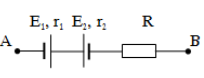
\includegraphics{../figs/VN11-2021-PH-TP015-1}
		\end{center}
	Trong đó: $\calE_1 = \SI{9}{V}$, $r_1=\SI{1.2}{\Omega}$, $\calE_2 = \SI{3}{V}$, $r_2=\SI{0.4}{\Omega}$, $R=\SI{28.4}{\Omega}$. Hiệu điện thế giữa hai đầu mạch là $U_\text{AB} = \SI{6}{V}$. Xác định chiều và độ lớn của cường độ dòng điện trong mạch.
		\begin{mcq}
			\item Chiều từ A sang B, độ lớn $I=\SI{0.4}{A}$.
			\item Chiều từ B sang A, độ lớn $I=\SI{0.4}{A}$.
			\item Chiều từ A sang B, độ lớn $I=\SI{0.6}{A}$.
			\item Chiều từ B sang A, độ lớn $I=\SI{0.6}{A}$.
		\end{mcq}
		
	}
	\loigiai
	{	\textbf{Đáp án: A.}
		
		Vì $\calE_1$ và $\calE_2$ mắc ngược chiều, mà $\calE_1 > \calE_2$ nên $\calE_1$ là nguồn, $\calE_2$ là máy thu. Do đó chiều dòng điện theo chiều từ A sang B.
		
		Cường độ dòng điện trong mạch:
		$$I=\dfrac{U_\text{AB} + \calE_1 - \calE_2}{R + r_1 + r_2} = \SI{0.4}{A}.$$
	}
	\item \mkstar{3}
	
	\cauhoi
	{Hai nguồn điện giống nhau, mỗi nguồn có suất điện động là 2 V, điện trở trong là $\SI{1}{\Omega}$, được mắc song song với nhau và nối với một điện trở ngoài $R$. Điện trở $R$ bằng bao nhiêu để cường độ dòng điện đi qua nó là 1 A?
		\begin{mcq}(4)
			\item $\SI{1.5}{\Omega}$.
			\item $\SI{1}{\Omega}$.
			\item $\SI{2}{\Omega}$.
			\item $\SI{3}{\Omega}$.
		\end{mcq}
		
	}
	\loigiai
	{	\textbf{Đáp án: A.}
		
		Suất điện động của nguồn:
		$$\calE_\text b = \calE = \SI{2}{V}.$$
		
		Điện trở trong của nguồn:
		$$r_\text b= \dfrac{r}{2} = \SI{0.5}{\Omega}$$
		
		Cường độ dòng điện đi qua $R$ là
		$$I=\dfrac{\calE_\text b}{R+r_\text b} = 1 \Rightarrow R = \SI{1.5}{\Omega}.$$
	}
	\item \mkstar{3}
	
	\cauhoi
	{Có 8 nguồn điện cùng loại với cùng suất điện động $\calE=\SI{2}{V}$ và điện trở trong $r=\SI{1}{\Omega}$. Mắc các nguồn thành bộ hỗn hợp đối xứng gồm hai dãy song song. Suất điện động $\calE_\text{b}$ và điện trở trong $r_\text{b}$ của bộ này bằng
		\begin{mcq}(2)
			\item $\calE_\text{b} = \SI{4}{V}$ và $r_\text{b} = \SI{2}{\Omega}$.
			\item $\calE_\text{b} = \SI{6}{V}$ và $r_\text{b} = \SI{4}{\Omega}$.
			\item $\calE_\text{b} = \SI{6}{V}$ và $r_\text{b} = \SI{1}{\Omega}$.
			\item $\calE_\text{b} = \SI{8}{V}$ và $r_\text{b} = \SI{2}{\Omega}$.
		\end{mcq}
		
	}
	\loigiai
	{	\textbf{Đáp án: D.}
		
		Suất điện động của bộ nguồn:
		$$\calE_\text b = 4 \calE = \SI{8}{V}.$$
		
		Điện trở trong của bộ nguồn:
		$$r_\text b = \dfrac{4r}{2} = 2r =\SI{2}{\Omega}.$$
	}
	\item \mkstar{3}
	
	\cauhoi
	{Có 24 nguồn điện giống nhau, suất điện động và điện trở trong của mỗi nguồn là $\calE=\SI{1.5}{V}$ và $r=\SI{0.5}{\Omega}$, mắc hỗn hợp đối xứng thành bốn dãy song song với nhau (mỗi dãy có 6 nguồn điện mắc nối tiếp). Suất điện động và điện trở trong của bộ nguồn này là
		\begin{mcq}(2)
			\item 6 V và $\SI{0.75}{\Omega}$.
			\item 9 V và $\SI{1.5}{\Omega}$.
			\item 6 V và $\SI{1.5}{\Omega}$.
			\item 9 V và $\SI{0.75}{\Omega}$.
		\end{mcq}
		
	}
	\loigiai
	{	\textbf{Đáp án: D.}
		
		Mắc 4 dãy, mỗi dãy có 6 nguồn nối tiếp:
		$$\calE_\text = 6\calE = \SI{9}{V}.$$
		$$r_\text b = \dfrac{6r}{4} = \SI{0.75}{\Omega}.$$
	}
	\item \mkstar{4}
	
	\cauhoi
	{Cho mạch điện như hình vẽ.
		\begin{center}
			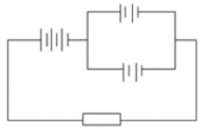
\includegraphics{../figs/VN11-2021-PH-TP015-2.png}
		\end{center}
	Mỗi pin có suất điện động $\calE=\SI{1.5}{V}$, $r=\SI{1}{\Omega}$, $R=\SI{3.5}{\Omega}$. Tìm cường độ dòng điện mạch ngoài.
		\begin{mcq}(4)
			\item $\SI{0.5}{A}$.
			\item 1 A.
			\item 2 A.
			\item $\SI{1.5}{A}$.
		\end{mcq}
		
	}
	\loigiai
	{	\textbf{Đáp án: B.}
		
		Xét đoạn mạch gồm 2 nhánh song song, mỗi nhánh gồm 2 nguồn nối tiếp thì ta có
		$$\calE_\text{ss} = 2 \calE;\ r_\text{ss} = \dfrac{2r}{2} = \SI{1}{\Omega}.$$
		
		Đoạn mạch gồm 3 nguồn nối tiếp thì ta có
		$$\calE_\text{nt} = 3 \calE = \SI{4.5}{V};\ r_\text{nt} = 3r = \SI{3}{\Omega}.$$
		$$\Rightarrow \calE = \calE_\text{ss} + \calE_\text{nt} = \SI{7.5}{V};\ r_\text{b} = r_\text{ss} + r_\text{nt} = \SI{4}{\Omega}.$$
		
		Cường độ dòng điện mạch ngoài là
		$$I=\dfrac{\calE_\text b}{R+ r_\text b} = \SI{1}{A}.$$
	}
\end{enumerate}

\whiteBGstarEnd

\loigiai
{
	\begin{center}
		\textbf{BẢNG ĐÁP ÁN}
	\end{center}
	\begin{center}
		\begin{tabular}{|m{2.8em}|m{2.8em}|m{2.8em}|m{2.8em}|m{2.8em}|m{2.8em}|m{2.8em}|m{2.8em}|m{2.8em}|m{2.8em}|}
			\hline
			1.A  & 2.C  & 3.A  & 4.D  & 5.B  & 6.C  & 7.A  & 8.D  & 9.C  & 10.D  \\
			\hline
			11.B  & 12.D  & 13.C  & 14.B  & 15.C  & 16.A  & 17.A  & 18.D  & 19.D  & 20.B  \\
			\hline
		\end{tabular}
	\end{center}
}
\section{Tự luận}
\begin{enumerate}[label=\bfseries Câu \arabic*:]
	\item \mkstar{1}
	
	\cauhoi{
		Dòng điện chạy qua đoạn mạch chứa nguồn điện có chiều như thế nào? Hãy trình bày các mối quan hệ trong đoạn mạch có chứa nguồn điện.
	}
	
	\loigiai{
		
		Dòng điện chạy qua đoạn mạch chứa nguồn điện có chiều đi ra từ cực dương và đi tới cực âm của nguồn điện.
		\begin{center}
			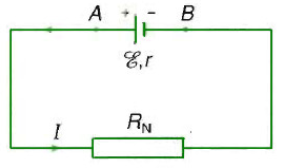
\includegraphics[scale=1]{../figs/VN11-2021-PH-TP015-3}
		\end{center}
	
		Trong đoạn mạch có chứa nguồn điện, mối quan hệ giữa các đại lượng được biểu diễn bằng công thức:
		$$U_\text{AB} = \calE - Ir,$$
		trong đó:
		\begin{itemize}
			\item $r$ là điện trở trong của nguồn điện;
			\item $\calE$ là suất điện động của nguồn điện.
		\end{itemize}
	}
	
	\item \mkstar{2}
	
	\cauhoi{
		Một bộ nguồn gồm hai nguồn điện mắc nối tiếp. Hai nguồn điện có suất điện động lần lượt là 5 V và 7 V. Tìm suất điện động của bộ nguồn.
	}
	
	\loigiai{
		
		Vì bộ nguồn mắc nối tiếp nên suất điện động của bộ nguồn là
		$$\calE = \calE_1 + \calE_2 = \SI{12}{V}.$$
	}
	\item \mkstar{3}
	
	\cauhoi{
		Một ắcquy có suất điện động và điện trở trong $\calE=\SI{6}{V}$ và $r=\SI{0.6}{\Omega}$. Sử dụng ắcquy này thắp sáng bóng đèn có ghi 6 V - 3 W. Tính cường độ dòng điện chạy trong mạch và hiệu điện thế giữa hai cực của ắcquy đó.
	}
	
	\loigiai{
		
		Điện trở của bóng đèn:
		$$R_\text{đ} = \dfrac{U_\text{đm}^2}{\calP_\text{đm}} = \SI{12}{\Omega}.$$
		
		Cường độ dòng điện chạy trong mạch:
		$$I=\dfrac{\calE}{R_\text{đ} + r} = \SI{0.476}{A}.$$
		
		Hiệu điện thế giữa hai cực của ắc quy khi đó:
		$$U=\calE - Ir = \SI{5.714}{V}.$$
	}
	\item \mkstar{4}
	
	\cauhoi{
		Cần dùng bao nhiêu pin $\SI{4.5}{V}$ - $\SI{1}{\Omega}$ mắc theo kiểu hỗn hợp để thắp cho bóng đèn 8 V - 8 W sáng bình thường?
	}
	
	\loigiai{
		
		Điện trở của đèn:
		$$R=\dfrac{U^2}{\calP} = \SI{8}{\Omega}.$$
		
		Giả sử pin mắc thành n dãy song song, mỗi dãy có m nguồn ghép nối tiếp.
		
		Ta có cường độ dòng điện đi qua mạch để đèn sáng bình thường là
		$$I=\dfrac{\calP}{U} = \SI{1}{A}.$$
		
		Suy ra:
		$$I=\dfrac{\calE_\text b}{R + r_\text b} = \dfrac{m \calE}{8 + \dfrac{mr}{n}} = \dfrac{4,5 mn}{m+8n} = \dfrac{4,5 p}{m+8n}\ (1).$$
		
		Thay $n=\dfrac{p}{m}$ vào (1) ta có:
		$$p=\dfrac{m^2}{4,5m - 8}.$$
		
		Vì $p$ dương nên $m> \dfrac{16}{9}$ hay $m>1$.
		$$n=\dfrac{p}{m} \geq 1 \Leftrightarrow \dfrac{m^2}{4,5m - 8} \geq 1 \Rightarrow m \leq 2,3$$
		
		Suy ra $m=2$, $n=2$ (có 4 pin được mắc thành 2 nhánh song song, mỗi nhánh gồm 2 pin nối tiếp).
	}
	\item \mkstar{4}
	
	\cauhoi{
		Một nguồn điện có suất điện động $\calE=\SI{1.5}{\Omega}$, điện trở trong $r=\SI{0.1}{\Omega}$. Mắc với hai cực của nguồn điện trở $R_1$ và $R_2$ thành mạch kín. Khi $R_1$ nối tiếp $R_2$ thì cường độ dòng điện qua mỗi điện trở là $\SI{1.5}{A}$. Khi $R_1$ song song $R_2$ thì cường độ dòng điện tổng cộng qua 2 điện trở là 5 A. Tìm giá trị của $R_1$ và $R_2$.
	}
	
	\loigiai{
		
		Khi $R_1$ nối tiếp $R_2$ thì cường độ dòng điện qua mỗi điện trở là
		$$I=\dfrac{\calE}{R_1 + R_2 + r}  \Rightarrow R_1 + R_2 = \SI{0.9}{\Omega}\ (*).$$
		
		Khi $R_1$ nối tiếp $R_2$ thì cường độ dòng điện tổng cộng qua 2 điện trở là
		$$I=\dfrac{\calE}{\dfrac{R_1 R_2}{R_1 + R_2} + r} \Rightarrow \dfrac{R_1 R_2}{R_1 + R_2} = \SI{0.2}{\Omega}\ (**).$$
		
		Từ $(*)$ và $(**)$, ta tính được:
		$$R_1 = \SI{0.6}{\Omega};\ R_2 = \SI{0.3}{\Omega}.$$
	}
	
\end{enumerate}